%% SW arkitektur: Deployment View

Deployment view skal illustrere hvor hvilke lag af software ligger på vores platforme. Devkit8000 kører Linux og har derfor flere softwarelag end PSoC'en.
 
\vspace{15 mm}

\begin{figure}[htbp] \centering
{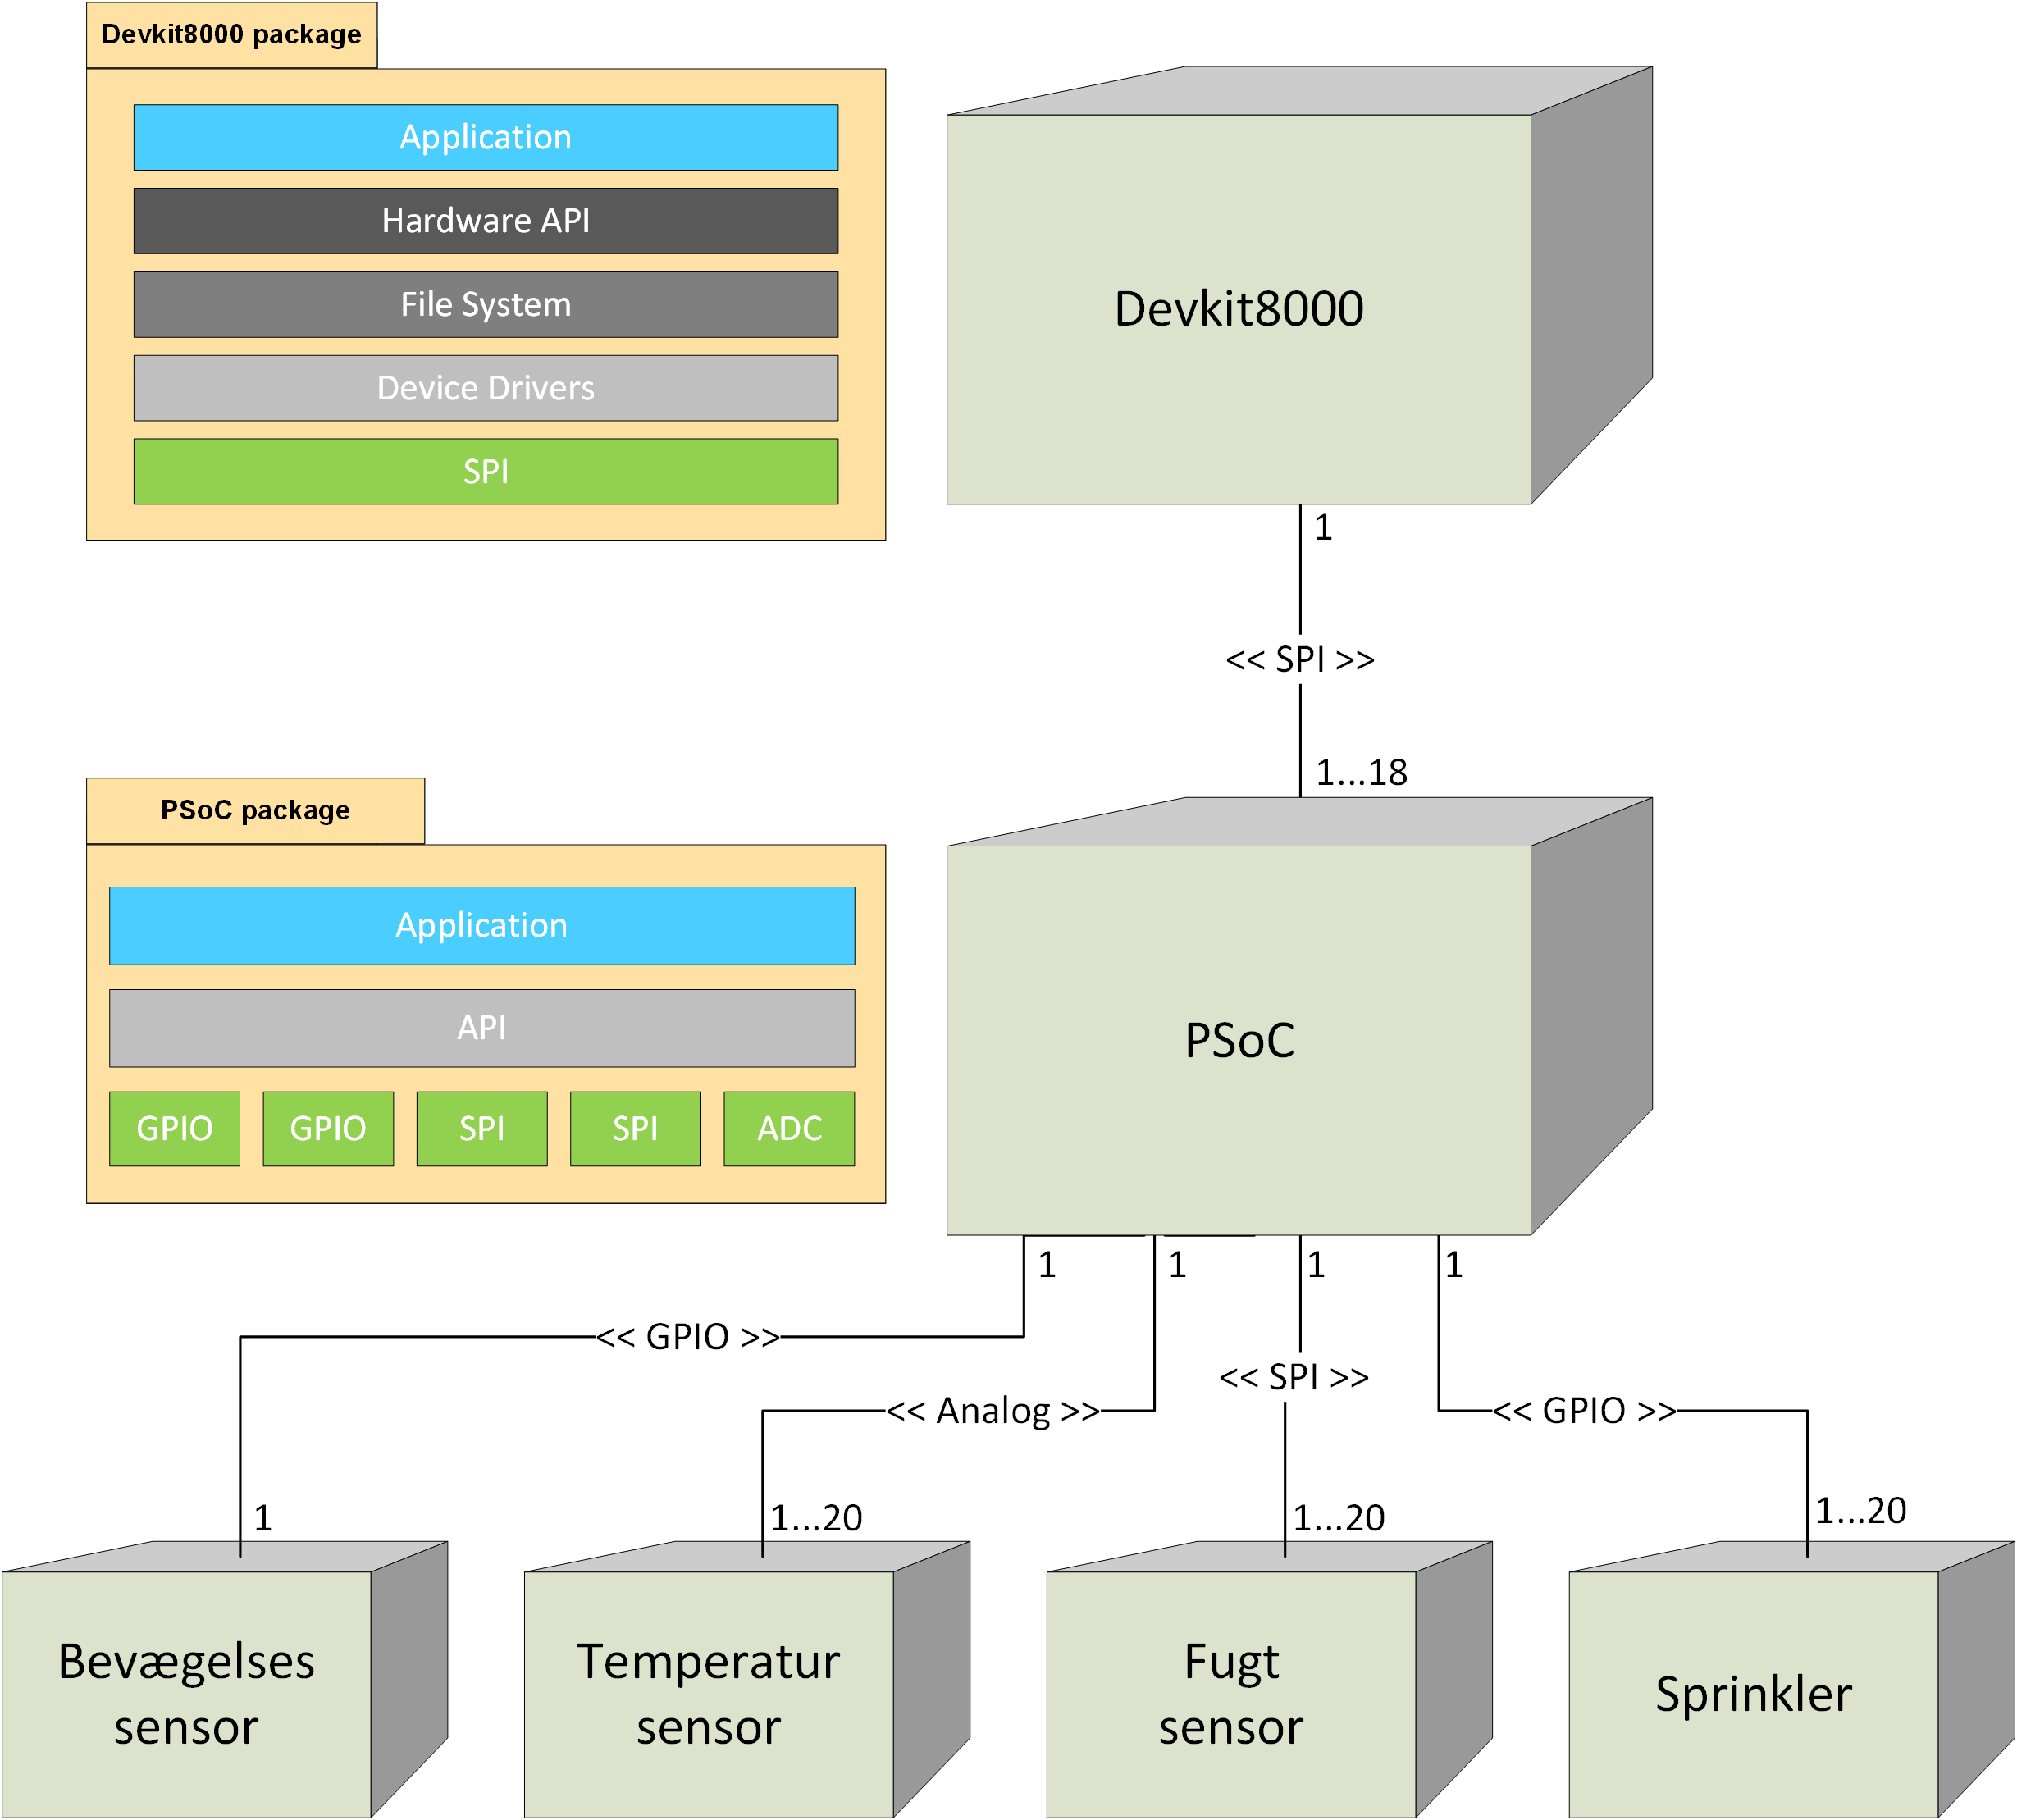
\includegraphics[scale=0.7]{filer/systemarkitektur/Deployment_model}}
\caption{Deployment model illustrerer de forskellige software og hardware(grønne) lag}
\label{fig:Deployment Model}
\end{figure}

\vspace{5 mm}

\subsubsection{Devkit8000}
\textit{Applications} laget består af al den software som har med brugeren at gøre, dvs. UI og tilhørende controllers. Applicationslaget tager imod input fra brugeren og reagerer på det enten ved at kalde nogle af sine egne controllers eller sende kommandoer til hardware APIen. Laget skal desuden få data fra nedenstående lag til at fremstå overskueligt over for brugeren.

\clearpage

\textit{Hardware API} laget består af almindelige klasser som gør brug af file systemets kommandoer som f.eks open og close.

\textit{File System} er en del af Linux systemet og håndteres der igennem.

\textit{Device Driver} laget består af den software som håndtere alt hardware input og output. Hardware proxys inklusiv. Det er dette lag hvor filsystemkommandoerne er defineret som bruges af \textit{File System}.

\textit{HW connection (grønne bokse)} laget viser hvilke hardware in/out forbindelser der er på Devkit8000.

\subsubsection{PSoC}

\textit{Applications} laget håndterer den indsamlede data som den får fra sensorene igennem API'en. Denne data sammensættes ifølge protokollen og sendes til API'en som får det sendt til devkittet. Laget skal også håndtere data fra devkittet til at konfigurere de parametre der styre automatiseringen af vandingen som applications-laget også håndterer.

\textit{API} laget består af den software som håndterer hardwaren, dvs. den tager imod input og får formateret det til noget læseligt til applications-laget. Derudover står den for at få sendt de informationer applicationslaget beder om på en effektiv og sikker måde.

\textit{HW connection (grønne bokse)} laget viser hvilke hardware in/out forbindelser der er til PSoC'en.